\documentclass[12pt,a4paper,oneside,openright]{report}
\usepackage{template/templateunibs}
\usepackage{setspace}
\usepackage[gen]{eurosym}
\usepackage{rotating} % sidewaytables
\usepackage{graphicx} % Required for inserting images
\usepackage{geometry}           % impostazione generale di pagina
\usepackage{emptypage}          % per lasciare bianche le pagine senza testo
\usepackage[babel]{csquotes}    % per la bibliografia
\usepackage{biblatex}           % per la bibliografia
\usepackage{lipsum}             % inserire lorem ipsum \lipsum[]
\usepackage{caption}            % per le didascalie
\usepackage{subcaption}

\usepackage{booktabs}           % per le tabelle
\usepackage{pdfpages}           % inserire pdf esterni

\usepackage{siunitx}            % unità di misura del SI
\sisetup{separate-uncertainty}

\usepackage{hyperref}           % collegamenti ipertestuali e segnalibri
\hypersetup{hidelinks}
\urlstyle{same}


%% COMMAND: figref adn tabref
\newcommand{\figref}[1]{Figura~\ref{#1}}
\newcommand{\tabref}[1]{Tabella~\ref{#1}}

\usepackage{xcolor}
%New colors defined below
\definecolor{codegreen}{rgb}{0,0.6,0}
\definecolor{codegray}{rgb}{0.5,0.5,0.5}
\definecolor{codepurple}{rgb}{0.58,0,0.82}
\definecolor{backcolour}{rgb}{0.95,0.95,0.92}
\definecolor{codeblack}{rgb}{0.95,0.95,0.92}
\definecolor{codemauve}{rgb}{0.58,0,0.82}

%\usepackage[colorlinks=true, allcolors=blue]{hyperref} % link
% codice programmi 
\usepackage{listings}
\lstset{ 
  backgroundcolor=\color{backcolour},   % choose the background color; you must add \usepackage{color} or \usepackage{xcolor}; should come as last argument
  basicstyle=\fontsize{10}{12}\ttfamily,
  %basicstyle=\footnotesize\ttfamily,        % the size of the fonts that are used for the code
  breakatwhitespace=false,         % sets if automatic breaks should only happen at whitespace
  breaklines=true,                 % sets automatic line breaking
  captionpos=b,                    % sets the caption-position to bottom
  commentstyle=\color{codegreen},    % comment style
  deletekeywords={...},            % if you want to delete keywords from the given language
  escapeinside={\%*}{*)},          % if you want to add LaTeX within your code
  extendedchars=true,              % lets you use non-ASCII characters; for 8-bits encodings only, does not work with UTF-8
  frame=single,	                   % adds a frame around the code
  keepspaces=true,                 % keeps spaces in text, useful for keeping indentation of code (possibly needs columns=flexible)
  keywordstyle=\color{codepurple},       % keyword style
  language=C,                 % the language of the code
  morekeywords={*,...},            % if you want to add more keywords to the set
  numbers=none,                    % where to put the line-numbers; possible values are (none, left, right)
  numbersep=5pt,                   % how far the line-numbers are from the code
  numberstyle=\tiny\color{codegray}, % the style that is used for the line-numbers
  rulecolor=\color{black},         % if not set, the frame-color may be changed on line-breaks within not-black text (e.g. comments (green here))
  showspaces=false,                % show spaces everywhere adding particular underscores; it overrides 'showstringspaces'
  showstringspaces=false,          % underline spaces within strings only
  showtabs=false,                  % show tabs within strings adding particular underscores
  stepnumber=5,                    % the step between two line-numbers. If it's 1, each line will be numbered
  stringstyle=\color{codemauve},     % string literal style
  tabsize=2,	                   % sets default tabsize to 2 spaces
  title=\lstname                   % show the filename of files included with \lstinputlisting; also try caption instead of title
}
\renewcommand\lstlistingname{Listato}
\renewcommand\lstlistlistingname{Listati}

\lstdefinestyle{codeAppendix}{
 basicstyle=\tiny\ttfamily\color{black}, % Colore del testo
  keywordstyle=\color{black}, % Colore delle parole chiave
  commentstyle=\color{black}, % Colore dei commenti
  stringstyle=\color{black}, % Colore delle stringhe
  numbers=left,
  numberstyle=\tiny\color{black}, % Colore dei numeri di riga
  breaklines=true,
  breakatwhitespace=true,
  showspaces=false,
  showstringspaces=false,
  showtabs=false,
  frame=none, % Nessuna cornice
  backgroundcolor=\color{white}, % Nessuno sfondo
  captionpos=b,
  tabsize=2
}



%% SDI: Comandi Template TESI
\newcommand{\defUniversita}[1]{\newcommand{\tesiUniversita}{#1}}
\newcommand{\defDipartimento}[1]{\newcommand{\tesiDipartimento}{#1}}
\newcommand{\defCdL}[1]{\newcommand{\tesiCdL}{#1}}

\newcommand{\defStudente}[1]{\newcommand{\tesiStudente}{#1}}
\newcommand{\defMatricola}[1]{\newcommand{\tesiMatricola}{#1}}
\newcommand{\defTitolo}[1]{\newcommand{\tesiTitolo}{#1}}
\newcommand{\defAA}[1]{\newcommand{\tesiAA}{#1}}

\newcommand{\defRelatoreA}[1]{\newcommand{\tesiRelatoreA}{#1}}
\newcommand{\defRelatoreB}[1]{\newcommand{\tesiRelatoreB}{#1}}
\newcommand{\defRelatoreC}[1]{\newcommand{\tesiRelatoreC}{#1}}

%% SDI: Pacchetti utilizzati per commenti e template.
%% A tesi conclusa dovrebbero poter essere eliminati.
\usepackage{comment}
\usepackage{lipsum}
\newenvironment{todo}{\color[rgb]{1.0,0.0,0.0}\noindent}{\newline}


\graphicspath{{images/}}     % dove trovare le immagini
\bibliography{bibliografia}  % dove trovare la bibliografia


%% BEGIN: Parametri Tesi
%% Definizione di alcuni paramteri per la compilazione del frontespizio.
\defDipartimento{Dipartimento di Ingegneria dell'Informazione}
\defCdL{Corso di Laurea in\\Ingegneria Elettronica}

\defStudente{Nome Cognome}
\defMatricola{123456789}
\defTitolo{Titolo della Tesi\\su più righe}
\defAA{2023/2024}

\defRelatoreA{Chiar.ma Prof.ssa Alessandra Flammini}
\defRelatoreB{Dott. Salvatore Dello Iacono}
%% END: Parametri Tesi


\begin{document}
\onehalfspacing

%\frontmatter
\newgeometry{left=20mm,right=20mm,top=25mm,bottom=20mm}
\begin{titlepage}
    \begin{center}

        \begin{figure}[t]
            \centering
            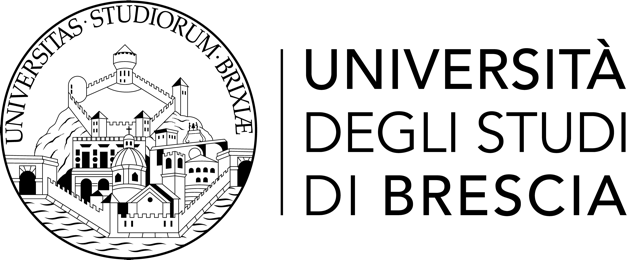
\includegraphics[width=72.4mm,height=30mm]{template/LogoUniBS.png}    
        \end{figure}

        \vspace*{10mm}

        {\fontsize{17}{17}\fontfamily{lmss}\selectfont
            \tesiDipartimento
        }

        \vspace*{10mm}

        {\fontsize{17}{17}\fontfamily{cmss}\selectfont
            \tesiCdL
        }    

        \vspace*{20mm}

        {\fontsize{20}{20}\fontfamily{lmss}\selectfont 
            \tesiTitolo
        }

    \end{center}

    \vfill

    \begin{flushleft}
        % inserisci il nome del relatore
        {\fontsize{17}{17}\fontfamily{lmss}\selectfont 
            \textbf{Relatore:} \tesiRelatoreA\\
            \vspace{0,5cm}
            \textbf{Correlatore:} \tesiRelatoreB \\
        }

    \end{flushleft}

    \vspace*{5mm}

    \begin{flushright}
        % completa con il tuo nome e matricola
        {\fontsize{17}{17}\fontfamily{lmss}\selectfont 
            Laureanda:\\
            \tesiStudente\\
            Matricola:\\
            \tesiMatricola\\
        }

    \end{flushright}


    \vspace*{5mm}

    \rule{0.8\textwidth}{0.4pt}
    \begin{center}
    {\fontsize{17}{17}\fontfamily{lmss}\selectfont 
        % specifica l'anno accademico
        Anno Accademico \tesiAA
    }
    \end{center}

\end{titlepage}
\restoregeometry

\leavevmode\thispagestyle{empty}\newpage
\tableofcontents            %  Creazione dell'indice

%\mainmatter                 % Corpo della tesi

\chapter*{Introduzione}
\addcontentsline{toc}{chapter}{Introduzione}
\label{chap:introduzione}

\lipsum[2-4]
\chapter{Titolo Primo Capitolo}
\label{chap:titolocapitolo01}

\lipsum[1]

\section{Primo Paragrafo}
\lipsum[2-3]


\subsection{Primo Sottoparagrafo}
\lipsum[4-5]

\subsection{Secondo Sottoparagrafo}
\lipsum[6-7]

\section{Secondo Paragrafo}
\lipsum[1-7]

\chapter{Titolo Capitolo 02}
\label{chap:titolocapitolo02}

\chapter{Titolo Capitolo 03}
\label{chap:titolocapitolo03}


%\backmatter
\chapter*{Conclusioni}
\addcontentsline{toc}{chapter}{Conclusioni}
\label{chap:conclusioni}

\lipsum[1-6]




\appendix 
\chapter{Esempi di Codice}
\label{chap:appendice}

L'appendice che contiene generalmente codice, schemi ecc deve essere scritta in piccolo ad esempio come segue:

\section{Fun Examples -- MATLAB Animation}
Taken from \href{https://github.com/mathworks/awesome-matlab-students/}{MathWorks -- Open Source and Community Projects}.

\begin{lstlisting}[language=Matlab,breaklines=true]
animateFrames();
function animateFrames()
    animFilename = 'Blender.gif'; % Output file name
    firstFrame = true;
    framesPerSecond = 24;
    delayTime = 1/framesPerSecond;

    % Create the gif
    for frame = 1:48
        drawframe(frame);
        fig = gcf();
        fig.Units = 'pixels';
        fig.Position(3:4) = [300,300];
        im = getframe(fig);
        [A,map] = rgb2ind(im.cdata,256);

        if firstFrame
            firstFrame = false;
            imwrite(A,map,animFilename, 'LoopCount', Inf, 'DelayTime', delayTime);
        else
            imwrite(A,map,animFilename, 'WriteMode', 'append', 'DelayTime', delayTime);
        end
    end
end
function drawframe(f)
    c=(sqrt(5)+1)/2;
    d=2*pi/c;
    alpha = interp1([0 48],[0 48*2*pi/12],f);
    theta = (1:600)*d;
    r = sqrt(theta);
    
    theta = theta + alpha;
    
    x = r.*cos(theta);
    y = r.*sin(theta);
    
    sz = 30*(1-(1:numel(x))/numel(x)) + 1;
    clr = sz;
    scatter(x,y,sz,clr,"filled")
    axis equal off
    axis(45*[-1 1 -1 1])
    set(gcf,Color=0.3*[1 1 1])
    
end
\end{lstlisting}
               % appendici

\printbibliography[heading=bibintoc]    % bibliografia

\chapter*{Ringraziamenti}

\begin{itshape}
\setlength\parindent{0pt}

I ringraziamenti sono opzionali... ma è consiglibile scriverli in corsivo e senza indentazione.


\lipsum[1]

\end{itshape}
          % ringraziamenti


\end{document}